\documentclass[pdftex,twoside,twocolumn,10pt,letterpaper]{article}
\usepackage{graphicx, subfigure, multirow, times, xspace}
\usepackage{url, amsfonts, verbatim, mathtools, color, soul}

\renewcommand{\ttdefault}{cmtt}
\usepackage{mdwlist}


\newenvironment{myitemize}
{
   \vspace{0mm}
    \begin{list}{$\bullet$ }{}
        \setlength{\topsep}{0em}
        \setlength{\parskip}{0pt}
        \setlength{\partopsep}{0pt}
        \setlength{\parsep}{0pt}
        \setlength{\itemsep}{1mm}
}
{
    \end{list}
}

\newcommand{\todo}[1]{\textbf{\textcolor{red}{TODO: #1}}}
\newcommand{\eg}{{\it e.g.,}\xspace}
\newcommand{\ie}{{\it i.e.,}\xspace}

% To make the FIXMEs go away, comment out this line...
\newcommand{\allnotes}[1]{}
% To make the FIXMEs go away, comment out this line...
\renewcommand{\allnotes}[1]{\textit{#1}}
\newcommand{\fixme}[1]{\allnotes{\bf\textcolor{red}{[#1]}}}
\newcommand{\panda}[1]{\allnotes{\bf\textcolor{blue}{[Panda: #1]}}}
\definecolor{comment-red}{rgb}{1,0,0}
\newcommand{\kay}[1]{\allnotes{\textnormal{\color{comment-red}{\textbf{KAY:#1}}}\unskip}}

\begin{document}
\title{\vspace{-1in}The Case for \begin{large}tinyTasks\end{large}}
\author{}
\date{}

\interfootnotelinepenalty=10000

\maketitle

\begin{quote}
  \textit{To see the world in a grain of sand...}\\
  \textit{-- William Blake}
\end{quote}
\section{Introduction}
Existing cluster compute frameworks like MapReduce, Spark, etc, rely on dividing a large unit of computation (a job)
into smaller, discrete units, \ie tasks. Tasks, and their storage analogs, blocks, are the atomic units of computation
on which extant cluster computing schedulers manage. Tasks provide a convenient atomic unit for which frameworks
provide scheduling, fault-tolerance, and other guarantees, \ie frameworks do not consider cases where a task partially
fails, nor do they schedule partial tasks. 

Most cluster frameworks use reasonably large blocks, and tasks, with a single task occasionally processing 1 GB of
data, and usually processing at least 64 MB of data. These large task, and block sizes are mostly dictated by the
prevalence of centralized metadata stores for distributed file systems, which make it necessary to reduce the amount of
metadata stored, and by the prevalence of distributed schedulers which require that scheduling be carried out at a
fairly coarse granularity, lest the centralized scheduler which lives on a single machine, be overwhelmed. In fact
prior work \fixme{cite facebook http://cloud.berkeley.edu/data/hdfs-scalability.pdf somehow} has argued that larger
blocks are a necessity for scaling such clusters.

However recent work on distributed filesystems~\cite{nightingale2012flat} has shown that one can efficiently
support a filesystem with much smaller block sizes using a distributed metadata store. At the same time, work on cluster
scheduling~\fixme{cite Kay's NSDI paper} has shown that distributed schedulers can schedule an extremely large number of
tasks with little or no increase in scheduling latency. Given these developments it is now feasible to schedule smaller
tasks than before. However the question of tasks sizes is far from resolved, while a wide range of sizes can now be accommodated,
what is an appropriate size for a task? In this paper we argue that smaller is better in this case, and make a case for
tiny tasks of a couple of hundred milliseconds each.

Tiny tasks build on the same intuition that has been used by network, and operating system designers, who found that
large indivisible chunks of work are inconvenient. Networks rely on dividing traffic into smaller packets, allowing for
increased utilization through statistical multiplexing, fairer sharing of bottle-necked links, and better load
balancing. Operating systems schedulers similarly rely on preemption as a means of running application ins small chunks
of a few milliseconds, allowing for fair allocation of resources amongst a wide
set of applications, including computationally intensive and interactive applications.

Some of the problems affecting data centers today are very similar to the problems solved by packets in networks, and
preemptible tasks in operating systems. Smaller tasks provide a mechanism similar to packets, where machines are
occupied for a much smaller time, thus helping with the following problems
\begin{itemize}
\item \textbf{Running batch jobs alongside interactive ones}: Running interactive
jobs is difficult in today's datacenters because long-running tasks for batch jobs may be
using the resources needed by an interactive job. Bursts of interactive jobs
cannot be serviced quickly, because they must wait for batch jobs to complete.
This problem frustrates data analysts trying to run real-time queries, and makes
running user-facing services alongside batch services impossible. Breaking large
jobs into millions of tiny tasks, each with runtime similar to the runtime for a
task in a user-facing service, eliminates this problem.
\item \textbf{Data Skew}: Data skew affects jobs in two ways: first, some tasks
may be processing far more data than other tasks, causing them to take much
longer; and second, congested network links due to one or more large jobs using
the same link can slow down other jobs reading data over the same link. Dividing
jobs into millions of tiny tasks dramatically improves load balancing to eliminate
this problem.
\item \textbf{Outliers}: Today's frameworks are plagued by outliers: tasks that
take as much as 10 or 100x longer than other tasks in the same job due to
resource contention at the machine or on the network or data skew.  If all tasks in a job execute in parallel, the job takes 10 or 100x longer than it would
have without the outlier, prompting a flurry of work on mitigating the outlier
problem ~\cite{blah,blah,blah}. On the other hand, if the job is broken into millions of tiny tasks (only a subset of which execute at any given time), a machine
that runs an outlier task will simply run fewer total tasks, rather than
stalling the completion time for the entire job. We have found that tiny tasks can reduce job
completion time by as much as a factor of 5.
\item \textbf{Misc Others that we'll probably eliminate:} Fragmentation (solves
lots of YARN's problems and simplifies scheduling)
\end{itemize}

While smaller tasks offer many benefits, there are certain kinds of tasks that might not benefit from such division. In
particular tasks which are not easily parallellizable, or whose performance increases sublinearly with increased
parallelism might in fact perform worse. In this paper we show that in many cases such tasks can be modified, by having
them use a framework provided scratch space, in a way that ameliorates this problem. We also show that a large class of
jobs can be readily converted to using smaller tasks, and demonstrate that tiny tasks still make sense in the presence
of a few longer jobs. In the next few sections, we list some of our assumptions, describe a few trends that motivate our
move towards smaller tasks, and then analyze the efficacy of such a move.

\section{Assumptions}
Our analysis targets large scale clusters running a mixture of analytical and interactive queries of the kind that are
prevalent today. While one could achieve results similar to ours through other means, we assume that cluster computing
frameworks have control over tasks, which are atomic units of work. A cluster compute framework can only schedule, or
kill processes at the granularity of a task, and either all of a task completes, and its output is used by other tasks
in the job, or none of a task finishes. Furthermore, we assume that a task cannot be preempted, it can only be killed.

We also assume, in a manner similar to what is available today, machines in a cluster have a certain number of
processing slots, and a certain amount of memory, that the cluster scheduler can allocate such memory and CPU, and can
get reasonable isolation from other tasks that are run on that machine. 

Finally our last assumption is that the network is reasonably fast, and full-bisection, such that the placement of tasks
is no longer a large concern. This is especially important as it allows for better load balancing, since tasks can be
placed on another machine more easily.

\section{Trends \& Motivation}

Common problems seen in datacenters. Probably need a graph for each one of these
\begin{myitemize}
  \item  Some tasks are very short/small and others are very large (in terms of
    resource usage) and long (in terms of time) \todo{Graph}.  
    Scheduling these is difficult; 

  \item Stragglers are exacerbated by the above problem~\todo{Graph}: if a task
    ends up on a machine with a large task consuming tons-o-resources, it will
    straggle

  \item Hot spots: there are hot spots in network usage, and also on machines
    that host popular data
\end{myitemize}

Make a table of problems caused by power-law distributions and papers about
them (should make this more concrete/compelling)

Datacenters and workloads are changing
\begin{myitemize}
  \item Focus is on main memory workloads, with need for low latency. Use the
    MapReduce$\rightarrow$Dremel$\rightarrow$Spark Streaming data here.
  \item Networks have grown to be fast making disk locality irrelevant. This
    means getting data from a remote location is fast. Further networks don't
    have a fixed overhead of transfer. Disk-based stuff uses 64MB to amortize
    that cost. \todo{Numbers ?}
  \item SSDs are becoming cheaper - Fast random access with low access time.
    With growing memory sizes + SSD, it is feasible to fetch most of the data
    without hitting the disk (local or remote).
  \item Need for low latency and ability to exploit fast-data access leads to
    tiny tasks
\end{myitemize}

\section{Melting Pot}
\panda{Need a better title, this is a discussion of what can be tiny taskable/what is needed. Also really this is a
potpurri at this time}
\begin{myitemize}
\item A tiny task is fundamentally a ``task'' that uses a small amount of input and runs relatively quickly. While one
can rely on programmers to make sure that the run time is small, it makes more sense to try and enforce this somehow,
and also provide tools to help the programmer. Further more running a taks on the same machine might provide some
benefits.
\item The lease/queuing thing for tasks
\item 
\end{myitemize}

\section{Benefits of Small Tasks}
\subsection{Running real-time and batch jobs together}
\kay{how can we quantify this?}
\subsection{How do small tasks affect stragglers?}
Breaking jobs into many waves of tiny tasks can improve completion time by 5x or more.  We assume task runtimes are exponentially distributed: some tasks take much longer than others due to resource contention on the machine, resource contention over the network, data skew, etc.  If tasks are all run in a single wave, the runtime of the job will be much longer than the mean task runtime, because the job is limited by the \emph{last} task to complete.  To measure the impact of breaking tasks up into a large number of tiny tasks, we assume jobs have a constant number of ''slots'' available, where a slot may represent a machine, or a fair share of the cluster allocated to the user who initiated the job.  we assume that if we break a task with mean runtime $x$ into k tiny tasks, each tiny task will have mean runtime $x/k$.  Figure~\ref{fig:outliers} demonstrates the impact of breaking a job with a single wave of tasks into $k$ times as many tiny tasks, for different values of $k$ (shown along the x-axis).  Response times are normalized relative to the response time for the job when run in a single wave.  We measure this impact for varying number of slots available to the job.  As expected, jobs with 1 slot see no improvement, but as the number of slots increases, jobs see as much as a 5x (eyeballed) improvement in response time from breaking tasks into tiny sub-tasks. This improvement justifies using a large number of tasks even if the overhead of starting a task is high; as long as the overhead of starting a task is less than 4x the task's completion time (we expect $<10$\% overhead), using tiny tasks will improve over running tasks in a single wave.

\begin{figure}[t]
\centering
\hspace{2ex}
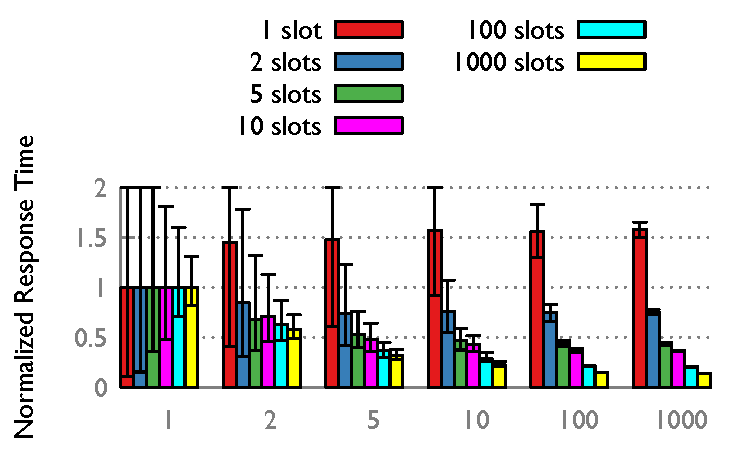
\includegraphics[width=0.5\textwidth]{figures/results_stragglers}
\vspace{-4ex}
\caption{Improvement in job completion time from breaking tasks into a large number of ``tiny tasks.'' \kay{need to fix 1-slot bars, which are screwed up, as well as nauseating colors}}
\vspace{-2ex}
\label{fig:outliers}
\end{figure}

TODO: use different original distributions of task duration

\subsection{How much do smaller tasks improve load balancing?}
two improvements on the load balancing front:
\begin{itemize}
\item File accesses: with smaller tasks, each task accesses a much smaller portion of a file.  In the context of Hadoop MapReduce, this would mean using much smaller HDFS file blocks.  With smaller blocks, the law of large numbers dictates that file accesses will be spread more evenly over machines than with large blocks.  To understand this affect, we use traces from Facebook's datacenter to obtain a distribution of the number of accesses per file.  We then randomly assign file blocks to machines, and measure the number of block accesses per machine, over 30 second intervals.\kay{should use smaller intervals? this would exacerbate affect, and you really care about how many accesses happen concurrently with yours, so 1s intervals could be realistic}  We divide files into smaller and smaller blocks (multiplier = 1 indicates block sizes equal to Facebook's current block size; multiplier = 10 indicates that we have block sizes 1/10th the size of Facebook's), to understand how smaller blocks improve load balancing.  With perfect load balancing, we would expect all machines to have the exact same number of file accesses.  Figure~\ref{fig:data_skew} demonstrates that even using 10 times as many tasks decreases 95th percentile machine load by 25\%\footnote{totally eyeballed from figure}.  \kay{we should simulate larger multipliers; my machine just died at 10}

\begin{figure}[t]
\centering
\hspace{2ex}
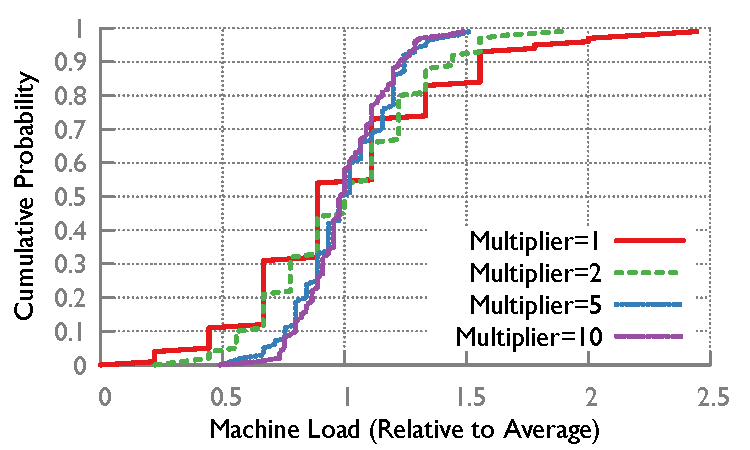
\includegraphics[width=0.5\textwidth]{figures/skew_results}
\vspace{-4ex}
\caption{Effect of decreasing file block size on the distribution of file accesses across machines.}
\vspace{-2ex}
\label{fig:data_skew}
\end{figure}

\item Network congestion: first, no huge flows (since all tasks are limited in how much data they use). This leads to essentially the same phenomenon as above.
\end{itemize}

\subsection{How do small tasks affect data skew?}
Many small tasks, so don't have to worry that one reducer (or other intermediate phase) has a ton of data.  Still need to worry about splitting very popular keys though...

\subsection{How does balance of tasks in a cluster (measured by queue length ?) change as we change granularity?}
\kay{Shivaram, what did you mean by this?}
\bibliographystyle{abbrv}
\bibliography{tiny-tasks}

\end{document}
